%//==============================--@--==============================//%
\clearpage
\subsection[1.2 Multiplexagem e comutação]{\hspace*{0.075 em}\raisebox{0.2 em}{$\pmb{\drsh}$} Multiplexagem e comutação}
\label{subsec:multiplexagem-e-comutação}


\subsubsection[1.2.1 Circuit Switching]{$\pmb{\rightarrow}$ Circuit Switching}

\begin{theo}[\underline{Circuit Switching}]{def:CircuitSwitching}\label{def:CircuitSwitching}

    ``In circuit-switched networks, \textbf{the resources needed along a path} to provide for communication between the end systems \textbf{are \textit{reserved}} for the duration of the communication session between the end systems.''\cite{Kurose2017}
\end{theo}

\begin{figure}[H]
    \centering
    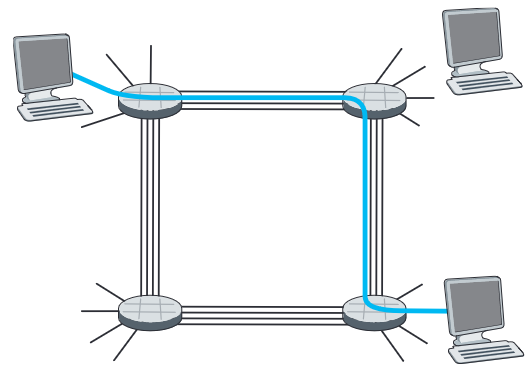
\includegraphics[width = 0.7\linewidth]{img/1/circuit-switching.png}
    \caption{Circuit Switching: ``In this network, the four circuit switches are interconnected by four links. Each of these links has four circuits, so that each link can support four simultaneous connections. The hosts (for example, PCs and workstations) are each directly connected to one of the switches. \textbf{When two hosts want to communicate, the network establishes a dedicated end-to-end connection between the two hosts.} Thus, in order for Host A to communicate with Host B, the network must first reserve one circuit on each of two links. \textbf{In this example, the dedicated end-to-end connection uses the second circuit in the first link and the fourth circuit in the second link.}''\cite{Kurose2017}}
    \label{fig:circuitswitching}
\end{figure}
\noindent A coordenação entre canal-subcanal de entrada e saída (referente à última frase da legenda da \hyperref[fig:circuitswitching]{Fig. 3}) é realizada através do uso de \textbf{tabelas de expedição} dinâmicas, que veremos mais adiante. 

\vspace{1 em}
\noindent Recorrendo novamente à \hyperref[fig:circuitswitching]{Fig. 3}, cada canal possui quatro circuitos, a velocidade trans- missão será um quarto da capacidade total do canal:

\begin{quote}
    ``Because each link has four circuits, for each link used by the end-to-end connection, the connection gets one fourth of the link’s total transmission capacity for the duration of the connection.''\cite{Kurose2017}
\end{quote}
$$
   \boxed{R_{\text{trans}} = \dfrac{R_{\text{link}}}{N}\; [\text{bps}]}
$$
\noindent Onde $N$ é o número de circuitos por canal (\textit{circuits} por \textit{link}).

%//==============================--@--==============================//%
\clearpage
\paragraph[1.2.1.1 Multiplexagem FDM]{$\pmb{\star}$ Multiplexagem FDM (\textit{frequency-division multiplexing})}\mbox{}

\begin{theo}[\underline{FDM}]{def:FDM}\label{def:FDM}
    ``With FDM, \textbf{the link dedicates a frequency band to each connection} for the duration of the connection''\cite{Kurose2017}
\end{theo}

\vspace{-0.75em}
\begin{figure}[H]
    \centering
    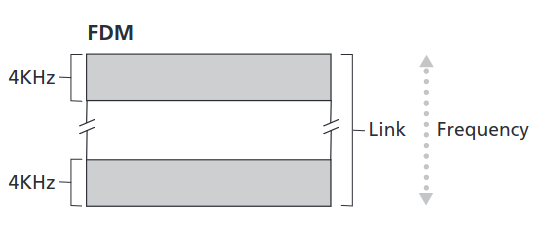
\includegraphics[width = 0.7\linewidth]{img/1/FDM.png}
    \caption{Vizualição das partições da banda de transmissão na multiplexagem de frequência}
    \label{fig:FDM}
\end{figure}

%//==============================--@--==============================//%
\paragraph[1.2.1.2 Multiplexagem TDM]{$\pmb{\star}$ Multiplexagem TDM (\textit{Time-division multiplexing})}\mbox{}

\begin{theo}[\underline{TDM}]{def:TDM}\label{def:TDM}
    ``For a TDM link, time is divided into frames of fixed duration, and each frame is divided into a fixed number of time slots. When the network establishes a connection across a link, the network dedicates one time slot in every frame to this connection.''\cite{Kurose2017}
\end{theo}

\begin{figure}[H]
    \centering
    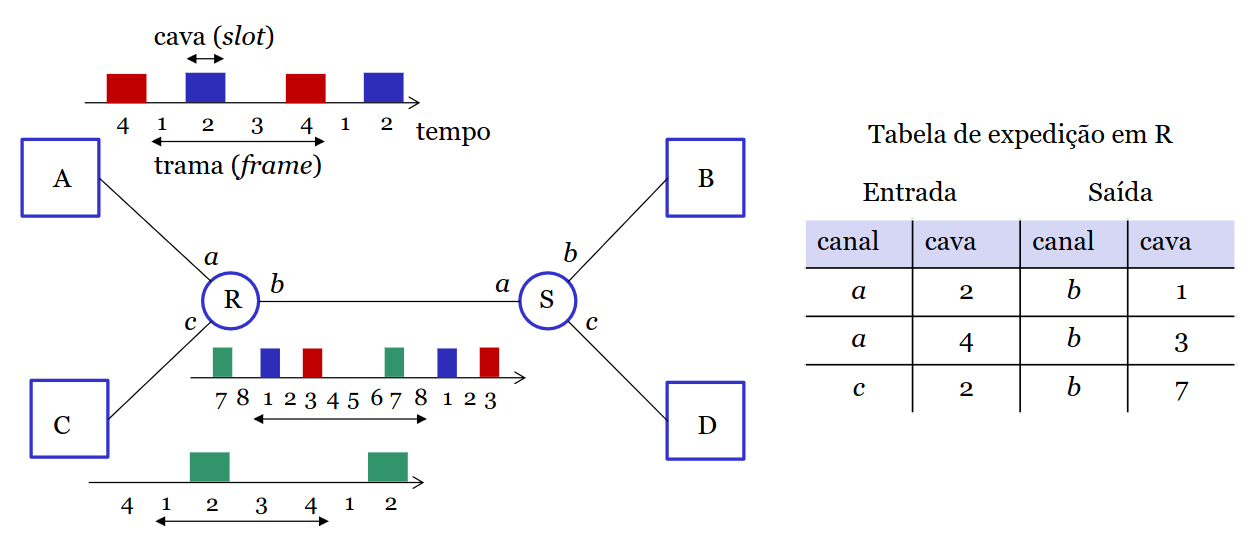
\includegraphics[width = 1\linewidth]{img/1/TDM.png}
    \caption{Time Division Mulplexing com respetiva tabela de expedição.}
    \label{fig:TDM}
\end{figure}

\noindent A informação é dividida no tempo em \textit{slots} (cavas), o conjunto de \textit{slots} origina uma estrutura denominada \textit{frame} (trama) de natureza períodica. A comutação entre canais é realizada através de tabelas de expedição que estabelecem associações entre canal e subcanal de entrada e saída:
\begin{enumerate}[label=$\rightarrow$]
    \item Na \hyperref[fig:TDM]{Fig. 5}, a informação a \textit{verde} comuta do canal $c$ para o $b$, sofrendo também uma comutação do subcanal 2 para o 7 (\textit{vide} tabela de expedição e a numerização dos slots). O mesmo processo verifica-se para a informação que comuta do canal $a$ para o canal $b$.
\end{enumerate}


%//==============================--@--==============================//%
\paragraph[1.2.1.3 Multiplexagem Determinística]{$\pmb{\star}$ Multiplexagem Determinística}\mbox{}\\[4pt]
O processo de \textit{circuit switching} é um método multiplexagem determinística (transmissão constante, certa, ``When the network establishes the circuit, it also reserves a constant transmission rate in the network’s links''\cite{Kurose2017})

{
\mdfsetup{linewidth=2pt}

\begin{mdframed}
\begin{enumerate}[label=$\blacktriangle$]
    \item Multiplexagem
        
        \vspace{-0.75em}
        \begin{itemize}
            \item Divisão de um canal em sub-canais de capacidades fixas (\textbf{TDM}, \textbf{FDM}, WDM, CDM).
        \end{itemize}
    \item Comutação (\textit{switching})
        
        \vspace{-0.75em}
        \begin{itemize}
            \item Circuito: concatenação de sub-canais ao longo de um caminho.
            \item Tabelas de expedição (fowarding table): associação entre pares de entrada (canal, sub-canal) e pares de saída (canal, sub-canal).
        \end{itemize}
        \item Circuitos dinâmicos:
        
        \vspace{-0.75em}
        \begin{itemize}
            \item Estabelecimento do circuito: atribuições de sub-canais em cada canal de um
                caminho e preenchimento das tabelas de expedição.
            \item Terminação do circuito: remoção das atribuições e limpeza das tabelas.
            \item Bloqueio se um canal não tiver um sub-canal disponível.
        \end{itemize}
\end{enumerate}
\end{mdframed}
}

%//==============================--@--==============================//%
\subsubsection[1.2.2 Packet Switching]{$\pmb{\rightarrow}$ Packet Switching}

\begin{theo}[\underline{Packet Switching}]{def:PacketSwitching}\label{def:PacketSwitching}

    ``\textbf{The source breaks long messages into smaller chunks of data known as \textit{packets}}. Between source and destination each packet travels through communication
    links and \textbf{\textit{packet switches}}---a router takes a packet arriving on one of its attached communication links and forwards that packet onto another one of its attached communication
links''\cite{Kurose2017}
\end{theo}

\renewcommand*{\thefootnote}{\fnsymbol{footnote}}
\footnotetext[1]{%
    ``Finally, there are two different ways to pronounce the word router, either as “rootor” or as “rowter,” and people waste a lot of time arguing over the proper pronunciation [Perlman 1999].''\cite{Kurose2017}
}
\renewcommand*{\thefootnote}{\arabic{footnote}}

\vspace{-1em}
\begin{figure}[H]
    \centering
    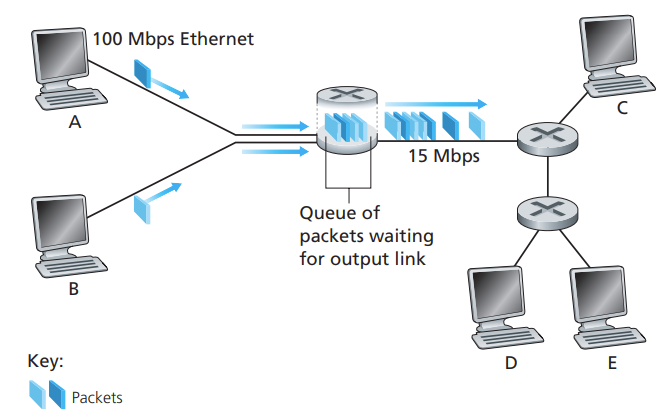
\includegraphics[width = 0.8\linewidth]{img/1/packet-switching.png}
    \caption{Packet Switching}
    \label{fig:PacketSwitching}
\end{figure}

\noindent Estes pacotes viajam com um ritmo igual ao ritmo total de transmissão do canal. Neste sentido, supondo o envio de um pacote de dimensão $L$ bits por um canal com capacidade $R$ bits/sec, o intervalo de tempo de transmissão é dado por:
$$
   \boxed{d_{\text{trans}} = \dfrac{L}{R}\; [\text{s}]}
$$
%//==============================--@--==============================//%
\paragraph[1.2.2.1 Store and Forward Transmission]{$\pmb{\star}$ Store and Forward Transmission}\mbox{}

\begin{theo}[\underline{Store and Forward Transmission}]{def:Store-For-Trans}\label{def:Store-For-Trans}
    ``Store-and-forward transmission means that \textbf{the packet switch \textit{must} receive the entire packet} before it can begin to transmit the first bit of the packet onto the outbound link.''\cite{Kurose2017}
\end{theo}
Pressupondo a transmissão de um pacote até um \textit{router} (\textit{packet switcher}) que aplica \textit{Store and Forward Transmission}, a subsequente comutação e transmissão para outro canal é apenas executada quando o \textit{router} possuir o pacote completo. Assim os bits já recebidos do pacote sofrem \textit{buffering} (são armazenados em fila de espera) até o \textit{router} possuir o pacote integral e proceder à sua transmissão.

\vspace{-1.2em}
\begin{figure}[H]
    \centering
    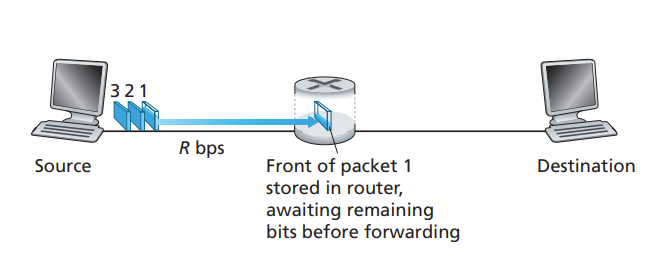
\includegraphics[width = 0.8\linewidth]{img/1/store-and-forward.png}
    \caption{Store and Forward transmission}
    \label{fig:Store-For}
\end{figure}

\noindent O tempo de espera resultante do processo de \textit{buffering} denomina-se de \textbf{\textit{queuing delay}}, $d_{\text{queue}}$. Este \textit{delay} é aleatório e está dependente do nível de \textbf{congestionamento} do canal (a taxa de chegada de pacotes a um comutador é superior à sua capacidade). Por outro lado o espaço da linha de espera é finito. Num caso extremo de congestionamento a linha de espera poderá encontrar-se totalmente preenchida, pacotes acabados de chegar poderão ser parcialmente ou totalmente perdidos, ocorre \textit{\textbf{packet loss}}.

%//==============================--@--==============================//%
\paragraph[1.2.2.2 Forwarding Tables and Routing Protocols]{$\pmb{\star}$ Forwarding Tables and Routing Protocols}\mbox{}

\begin{theo}[\underline{Forwarding Tables}]{def:Ftables}\label{def:Ftables}
    ``(...) Each router has a forwarding table that maps destination addresses (or portions of the destination addresses) to that router’s outbound links. \textbf{When a packet arrives at a router, the router examines the address and searches its \textit{forwarding table}}, using this destination address, \textbf{to find the appropriate outbound link}.''\cite{Kurose2017}
\end{theo}
\clearpage
As tabelas de expedição (\textit{forwarding tables}, localizadas nos cabeçalhos dos pacotes) são elaboradas automaticamente com recurso a \textit{\textbf{routing protocols}}:

\begin{quote}
    ``A \textbf{\textit{routing protocol}} may, for example, determine the shortest path from each router to each destination and use the shortest path results to configure the forwarding tables in the routers.''\cite{Kurose2017}
\end{quote}

%//==============================--@--==============================//%
\paragraph[1.2.2.3 Multiplexagem Estatística]{$\pmb{\star}$ Multiplexagem Estatística}\mbox{}\\[4pt]
\noindent O processo de \textit{packet switching} é um método de multiplexagem estatística---decorre da partilha assíncrona de um canal entre pacotes e obedece à política \textit{first come first served} (a transmissão de pacotes é realizada por ordem de chegada). A qualidade estatística refere-se ao caráter aleatória do congestionamento e \textit{rate} de transmissão:

{
\mdfsetup{linewidth=2pt}

\begin{mdframed}
    \begin{enumerate}[label=$\blacktriangle$]
        \item Multiplexagem
    
            \vspace{-0.75em}
            \begin{itemize}
                \item Mensagens e \textit{data streams} são divididas em pacotes (\textit{packages}) de pequena dimensão.
                \item Partilha assíncrona (no tempo) de um canal entre pacotes.
                \item Cabeçalhos distinguem os pacotes.
                \item Os cabeçalhos (\textit{headers}) dos pacotes contêm informação que permite o seu
                posterior reagrupamento nos dados originais.
            \end{itemize}
        \item Comutação
    
            \vspace{-0.75em}
            \begin{itemize}
                \item \textit{Store-and-forward}: cada mensagem é recebida na
                totalidade antes de ser expedida.
                \item As tabelas de expedição estabelecem a localização do subsequente \textit{outbound-link} através da associação entre terminais de entrada e saída.
            \end{itemize}
        \item \textbf{Equidade} na partilha dos recursos de transmissão e comutação (\textit{switching}).
        \item \textbf{Congestionamento} se a taxa de chegada de mensagens a um comutador for
    superior à capacidade deste, conduzindo a atrasos e, possivel perdas.
    \end{enumerate}%adoro-te :3
\end{mdframed}
}

\noindent \textbf{Nota:} Ao não executar a partição de dados em pacotes de menor tamanho a transmissão fica sujeita a períodos de \textbf{inequidade} (\textit{starvation}): quando uma mensagem longa impede o despacho de
mensagens curtas.

%//==============================--@--==============================//%
\subsubsection[1.2.3 Circuit Switching vs. Packet Switching]{$\pmb{\rightarrow}$ Circuit Switching vs. Packet Switching}
\vspace{-1 em}
\begin{table}[H]
    \begin{tabularx}{\linewidth}{>{\parskip1ex}X@{\kern4\tabcolsep}>{\parskip1ex}X}
    \toprule
    \hfil\bfseries Circuit Switching
    &
    \hfil\bfseries Packet Switching
    \\\cmidrule(r{3\tabcolsep}){1-1}\cmidrule(l{-\tabcolsep}){2-2}
    
    %% separated by empty line or \par
    Ideal para aplicações que exigem comu- nicação confiável/determinística, como as redes telefónicas.\par
    Fornece uma qualidade de serviço consis- tente.\par
    Requer um caminho dedicado durante toda a sessão de comunicação, mesmo durante períodos de inatividade.
    &
    
    %% separated by empty line or \par
    Garante flexibilidade e eficiência para redes com um elevado número de uti- lizadores.\par
    Experiência de comunicação imprevisível, graças à política de \textit{first come first served}.\par
    Mais simples, mais eficiente (em termos de recursos), e menos dispendiosa de implementar
    \\\bottomrule
    \end{tabularx}
    \caption{Pros \& cons dos tipos de comutação abordados.}
\end{table}
%//==============================--@--==============================//%
\subsubsection[1.2.4 Virtual Circuits]{$\pmb{\rightarrow}$ Virtual Circuits}

\begin{theo}[\underline{Virtual Circuits}]{def:virtual-circuits}\label{def:virtual-circuits}
    ``Virtual circuits provide a logical, \textbf{pre-determined path within a packet-switched network}, such as Frame Relay, Asynchronous Transfer Mode (ATM), and Multiprotocol Label Switching (MPLS) networks. Virtual circuits use statistical multiplexing, which is an intrinsic feature of packet-switched networks, allowing multiple virtual circuits to share the same physical links and resources, leading to better utilization of network resources and increased efficiency.'' $[$\textbf{?}$]$
\end{theo}

\vspace{-1em}
\begin{figure}[H]
    \centering
    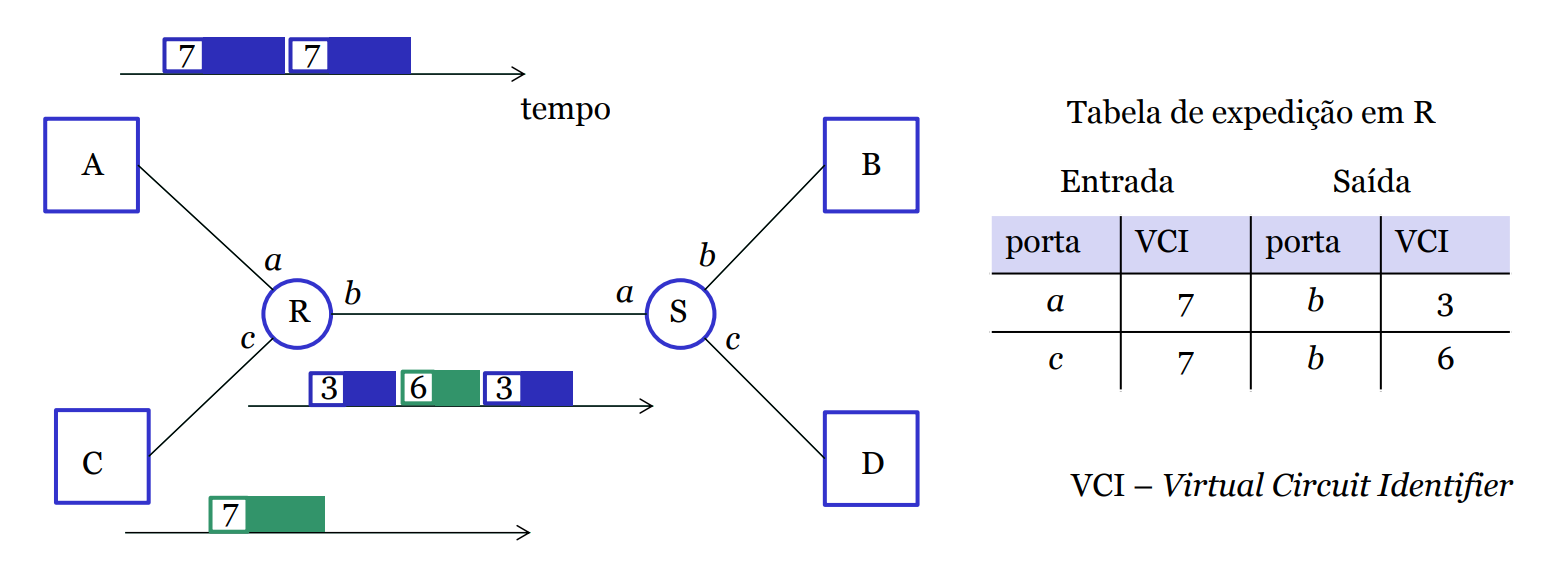
\includegraphics[width = 0.9\linewidth]{img/1/virtual-circuits.png}
    \caption{Circuitos virtuais.\protect\cite{slidesSobrinho}}
    \label{fig:virtual-circuits}
\end{figure}

\noindent While virtual circuits do not reserve a fixed bandwidth like traditional circuit-switched networks, they can offer certain advantages such as:
\begin{itemize}[label=$\blacktriangle$]
    \item \textbf{Established path}, which may lead to more consistent performance compared to purely connectionless packet switching.
    \item \textbf{In-order delivery} of packets, as they follow the same pre-determined path.
\end{itemize}

\noindent By allowing multiple virtual circuits to share the same physical links and resources, virtual circuits provide greater flexibility and efficiency compared to traditional circuit-switched networks.